\documentclass[12pt]{article}
 
\usepackage[utf8x]{inputenc}
\usepackage[brazilian]{babel}
\usepackage{fontenc}
\usepackage{graphicx} 
\usepackage{listings}
\usepackage{xcolor}
\usepackage{indentfirst}
\usepackage{pdflscape}
%\usepackage[defaultmono]{inconsolata}
\usepackage[bottom=3cm,top=3cm,left=3cm,right=3cm]{geometry} 
\usepackage[pdftex]{hyperref} %permitir \url

%varias figuras
%\usepackage[demo]{graphicx}
\usepackage{subfig}

%\renewcommand*\rmdefault{inconsolata}


\lstset{
    language=java,
    keywordstyle=\bfseries\ttfamily\color[rgb]{0,0,1},
    identifierstyle=\ttfamily,
    commentstyle=\color[rgb]{0.133,0.545,0.133},
    stringstyle=\ttfamily\color[rgb]{0.627,0.126,0.941},
    showstringspaces=false,
    basicstyle=\small,
    tabsize=2,
    breaklines=true,
    frame=single
}

\title{Programação Orientada a Objetos \\ Trem vol. 3}

\author{David Sena Oliveira}

\date{Quixadá, Outubro de 2014}

\renewcommand{\tt}[1]{\lstinline|#1|}
\renewcommand{\bf}[1]{\textbf{#1}}
\newcommand{\code}[1]{\emph{#1}}
\newcommand{\n}{\lstinline|\n|}

\begin{document}

\begin{figure}
\centering

\includegraphics[width=0.4\linewidth]{./imagens/ufc}
\label{fig:ufc}
\end{figure}

\maketitle

\section{Descrição}

Nesse terceiro volume do Trem serão apresentadas várias pequenas modificações no volume dois. Você criará uma pessoa Fresca que não fica em vagões próximos de animais e até tem um vagão preferencial pra ela.  Você implementará um tipo de pessoa que gosta de andar nos vagões com os animais caso seja possível. Conseguirá organizar e modularizar refatorando seu código parte a parte.

\begin{figure}
\subfloat[Fresco]{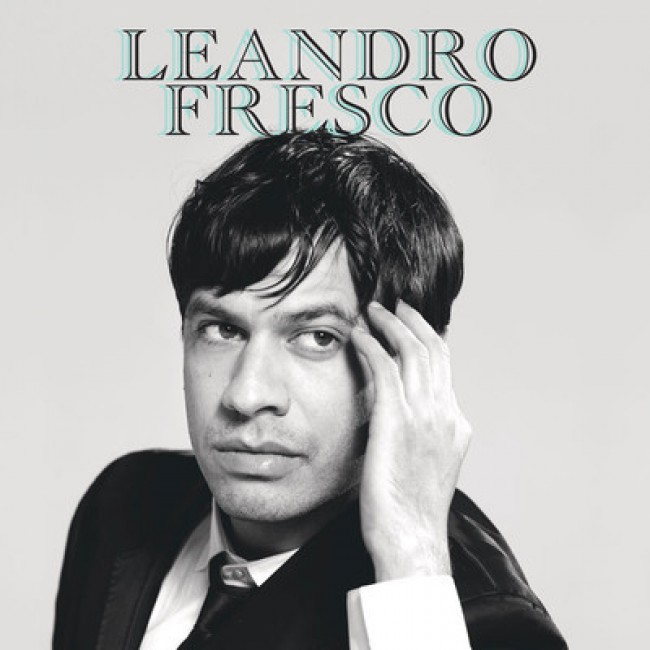
\includegraphics[width = 1.5in]{./imagens/fresco}}
\subfloat[VagaoLuxo]{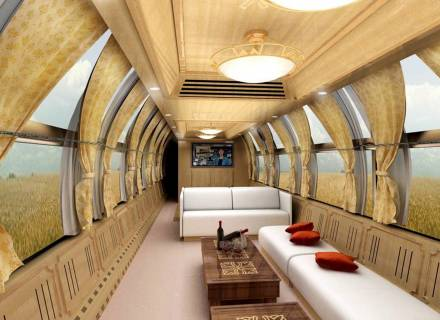
\includegraphics[width = 1.5in]{./imagens/luxo}}
\subfloat[GreenPeace]{
\includegraphics[width = 1.5in]{./imagens/green}}
\subfloat[Juntos]{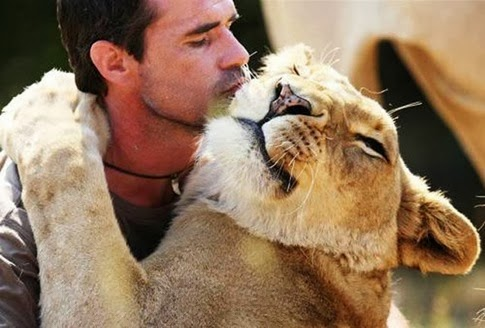
\includegraphics[width = 1.5in]{./imagens/pessoas_animais}}
\caption*{}
\end{figure}

Ao final desse artigo você vai encontrar o controlador, os diagrama de classes e a saída esperada da junção de todas as seções. Não tente fazer tudo ao mesmo tempo. A cada nova seção tente fazer seu código funcionar.
\section{Pessoas Frescas}

Nossos vagões normais não possuem ar condicionado. Isso faz com que os vagões de pessoas que ficam
atrás dos vagões de animais consigam sentir um pouco de mal cheiro que vem dos vagões de animais.
Pessoas frescas exigem ficar a uma distância mínima de qualquer vagão de animais a sua frente
ou não aceitam embarcar no trem.

Implemente a classe Fresca herdando da classe Pessoa. Ela deve ter um atributo \tt{int frescura} que determina
a quantos vagões de distancia ela deve estar de um vagão de animais a sua frente. Um nível de frescura 1 indica que deve haver um vagão de pessoas ao menos entre o vagão dela e o primeiro vagão de animais a sua frente.

Implemente os seguintes construtores e métodos.

\begin{lstlisting}
	private void init(int frescura){
    public Fresca(String nome); //inicia frescura em 1
    public Fresca(String nome, int frescura);
    public int getFrescura();
}
\end{lstlisting}{

O método init é usado pelos construtores para não haver replicação de código nos
construtores.

Você precisará alterar o método embarcar do trem para tentar embarcar a Fresca apenas nos vagões válidos.
Se tiver muita dificuldade com a lógica de programação, fixe o nível de frescura em 1 e implemente apenas
para esse nível de frescura.

Você pode criar também um novo vagão de Luxo que estende de Vagão de Pessoas. Ele tem sempre duas vagas fixas. Neste vagão, porém, apenas os frescos devem poder embarcar, desde que são mais caros e tem ar condicionado, o que impede o cheiro do animais, independente da sua localização em relação aos outros vagões. Se preferir, crie uma classe abstrata intermediária VagaoGente e coloque os métodos comuns entre VagaoPessoa e VagaoLuxo. 

Se existirem vagões de Luxo, essa será a escolha preferencial dos Frescos. Se não existirem, ou estiverem lotados, os frescos
deveram ser embarcados de acordo com seu nível de frescura nos vagões de Pessoas. No embarcar do Trem utilize \tt{instanceof} para descobrir qual
o tipo dos vagões.

Implemente um controlador que teste a inclusão das pessoas frescas e do VagaoLuxo. Certifique-se que apenas os frescos embarquem no Vagao de Luxo.

Você não precisa alterar os métodos \tt{toString()} da fresca. No vagão de luxo use o char @ para determinar o inicio e o fim
do vagão.

\section{GreenPeace}
Uma pessoa do GreenPeace estende de Pessoa. O GreenPeace deseja ser embarcado no vagão de animais. Isso nos traz um problema.
Vagões de animais só permitem Passageiros que sejam instancias de Animais, desde que ele exige uma função \tt{int getPeso()} para lidar com a alocação.

Uma solução é criar uma interface \tt{Pesavel} que estende da interface \tt{Passageiro} e que possui um único método: \tt{int getPeso();}. 

Faça tanto Animal quanto GreenPeace implementarem Pesavel.
Altere o Vagão de Animais para ser um vagão de Carga e trabalhar com objetos Pesáveis.

Faça dois construtores para o GreenPeace, um que recebe apenas o nome e inicializa com peso default de 70 kg, e outro
que recebe nome e peso.
Altere o toString() to GreenPeace para adicionar o peso ao final da String.

A lógica de embarque do GreenPeace é simples, caso ele caiba em algum vagão de animais ele embarca nesse vagão de animal. Caso contrário, ele tenta embarcar normal no vagão de pessoas.
Altere o método embarcar do trem para lidar com o caso de passageiros GreenPeace.

\section{Alternativa ao instanceof}
Usar \tt{instanceof} para verificar o tipo de uma classe é dispendioso. Deve ser usado a menor quantidade de vezes possível.
Em nosso código precisamos comparar várias vezes se uma classe é de um tipo específico. 

Para uma solução simples podemos criar enumerações para nossos tipos. Em especial os vagões e os passageiros.
Para organizar e agrupar criaremos uma classe \tt{public Types} que irá contem \tt{public enum}s.

Observe que em alguns casos especiais vamos precisar do instanceof. Quando exigir a escolha múltiplas opções talvez o melhor seja
o instanceof. Exemplo: Pesavel é tanto Green quanto Animal, e Pessoa também é o Green e o Fresco.

\begin{lstlisting}[float=ht]
public class Types {
	public enum VagaoType{VPESSOAS, VCARGA, VFRESCOS};
	public enum PassType{ANIMAL, FRESCA, PESSOA, GREEN};
}
\end{lstlisting}

Devemos adicionar na classe Vagao e interface Pessoa o \tt{getType()} correspondente. Os tipos devem ser inicializados nos construtores. Ex: Pessoa possui um atributo \tt{Types.PassageiroType type} que no construtor é iniciador com
\tt{this.type = Types.PassageiroType.PESSOA}. 

Ao invés de utilizar os instanceofs, faça uma verificação de tipo através do getType quando possível. A cada nova classe que cria um novo tipo, atualize a classe \bf{Types} ou outros tipos ou outras valores.

A classe Enumset do Java permitiria se livrar completamente do instanceof do nosso caso. Ela funciona como as implementações de enum bit field no C++. Por ela podemos definir que GreenPeace é do tipo PESAVEL e também PESSOA e também GREEN. Podemos perguntar ao receber um passageiro se seu tipo \bf{contém} PESAVEL. Essa implementação é opcional, tente implementar depois se tiver curiosidade.

\section{Lógica}
Como você deve ter percebido, o embarcar deve ter ficado uma bagunça. Imagine se começarmos a incluir mais pessoas
e lógicas de embarque. Precisamos organizar isso. Mesmo que criássemos uma classe pra gerenciar o embarque, 
a inclusão de cada novo tipo de passageiro exigiria mexer nessa classe. A lógica é um algoritmo e está relacionada
a um passageiro. Cada passageiro precisa de uma lógica de embarque.

Uma solução é criar uma interface Logica que tenta realizar o embarque de um passageiro no trem.
Crie um \tt{package} logica para colocar a interface \tt{Logica} e as implementações.

\begin{lstlisting}[float=ht]
public interface Logica {
    public boolean embarcarNoTrem(Vector<Vagao> vagoes, Passageiro passageiro);
}
\end{lstlisting}

Cada passageiro deve ter uma lógica. Essa lógica é obtida através do método \tt{Logica getLogica()} que foi adicionado
ao passageiro. 

Nas implementações do Passageiro adicione um atributo Logica que deve ser inicializado no construtor. A \bf{Pessoa} deve instanciar uma \bf{Logica} do tipo \bf{LogicaPessoa}. A LogicaPessoa procura por vagões de pessoas e tenta adicionar-los no vagão. 

Como as checagens e verificações de tipo foram trazidas para o objeto lógica, na classe abstrata \bf{Vagao} não 
faz mais sentido manter o método \bf{boolean embarcar(Passageiro passageiro)}. Essa assinatura força a verificação do tipo Pessoa dentro do \bf{VagaoPessoa}, o que nos faria verificar o tipo duas vezes, uma na classe Logica e outra no Vagão. 

Assim, cada classe específica pode fazer um método com assinatura específica ao seu tipo. Na classe \bf{VagaoPessoas} colocamos o método \tt{boolean embarcar(Pessoa pessoa)} e na classe \bf{VagaoCarga} colocamos o método \tt{boolean embarcar(Pesavel pesavel)}.
Na classe \tt{VagaoVIP} colocamos apenas para aceitar Frescos. A logica do vagão se limita a avaliar a capacidade e inserir.

Implemente as lógicas para Pessoa, Fresca, Pesavel, GreenPeace e corrija os métodos embarcar dos vagões. O método embarcar
do trem, que tenta embarcar o passageiro, chama 
\tt{passageiro.getLogica().embarcarNoTrem(vagoes, passageiro)} para tentar realizar o embarque.

Tente reaproveitar o código entre os classes Lógica. O GreenPeace utiliza tanto a lógica Pesável quanto Pessoa. Tente usar a regra de nunca se repetir ou duplicar código.

Para você que quer aprender mais, essa modelagem que usamos é um padrão chamado
Strategy que consistem em definir uma família de algoritmos e encapsulá-los dentro
de uma classe permitindo que possam ser trocados. 

Se tiver curiosidade, também pode usar a classe enumeração do Java para colocar
diferentes implementações do \bf{embarcarNoTrem()} em um único arquivo. Mais detalhes em \url{http://pt.wikipedia.org/wiki/Strategy}.

\section{Refatorando Passageiro}
Passageiro passou a ter vários métodos e vários atributos em comum.
Talvez seja adequado transformar Passageiro em classe abstrata e trazer
os atributos e gets comuns para interface. Faça as alterações necessárias nas classes.

Observe que a interface Pesavel não poderá mais extender Passageiros e algumas alterações serão necessárias no Vagão de Carga. Improvise. Na Listings \ref{Passageiro}, a nova classe Passageiro com todas as alterações anteriores.

Num sistema maior, essa refatoração trás mais prejuízos que ganhos. Aqui ela economiza um pouco de código, mas cria dependências indesejada. Faça para aprender, depois desfaça. Observe que ser um passageiro é um estado temporário. A pessoa ou animal se torna passageiro quando entra no Trem e deixa de sê-lo quando sai. O uso de interface é mais adequado nesses casos. Tente estudar um pouco sobre quando usar herança x interface x composição. Talvez esse link te ajude
\url{http://www2.lsd.ufcg.edu.br/~nazareno/ensino/si1/06.InterfacePolimorfismoHerancaComposicao.pdf}

\begin{lstlisting}[label=Passageiro, caption=Passageiro, float=ht]
public abstract class Passageiro {
	protected int id;
	protected Logica logica;
	protected Types.PassType type;
	
	public int getId(){
		return id;
	}
	public void setId(int id){
		this.id = id;
	}
	/**
	 * @return Todos os atributos da classe no formato
	 * id:nome:outro:outro
	 */
	public abstract String toString();
	
	public Logica getLogica(){
		return logica;
	}
	public Types.PassType getType(){
		return type;
	}
}
\end{lstlisting}

\section{Finalizando}

Se forem implementados todas as seções desse artigo, o controlador apresentado na Listings \ref{controlador} gera a saída vista no Listings \ref{output}. O diagrama de classes completo pode ser visto nas Figuras \ref{fig:diagrama} e \ref{fig:logicas}.


\begin{landscape}
%\begin{sidewaysfigure}
\begin{figure}
\centering
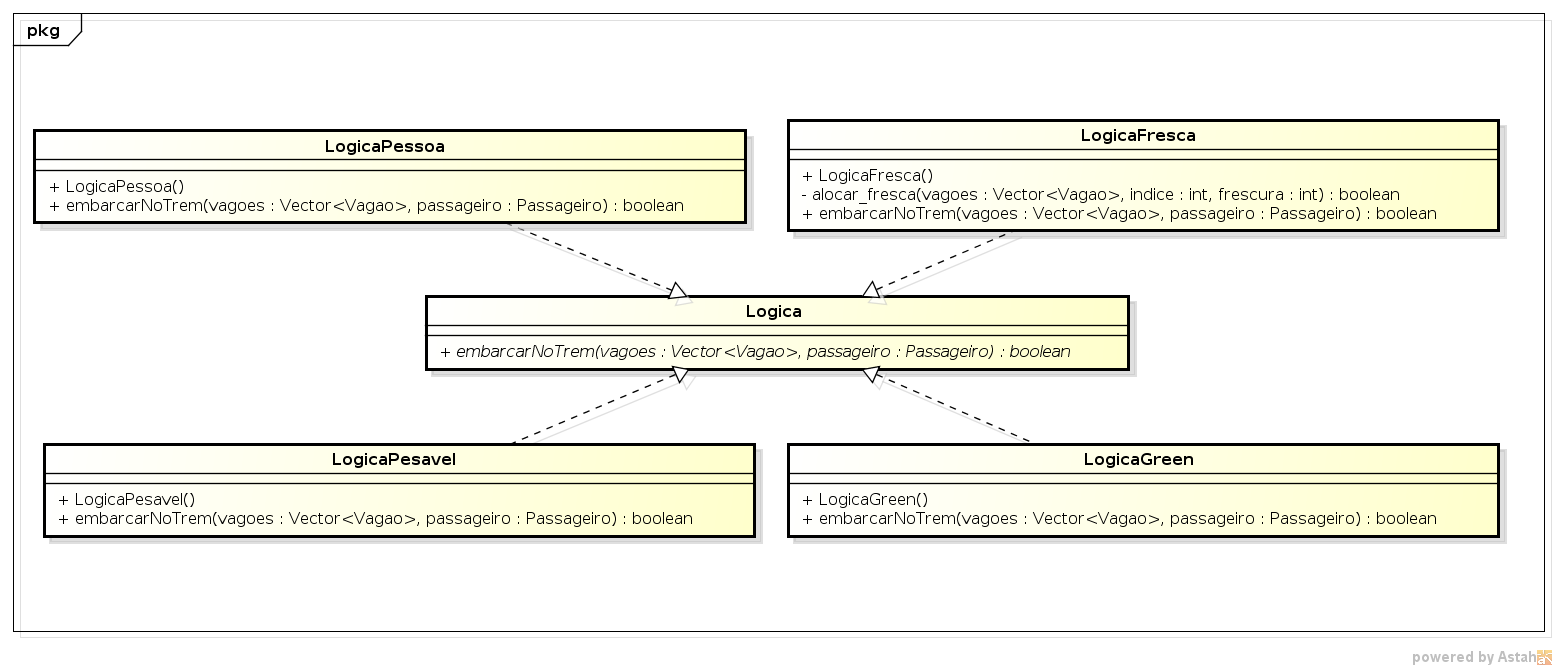
\includegraphics[width=1.1\linewidth]{./logicas}
\caption{Diagrama com as Lógicas}
\label{fig:logicas}
\end{figure}
%\end{sidewaysfigure}
\end{landscape}

\begin{landscape}
%\begin{sidewaysfigure}
\begin{figure}
\centering
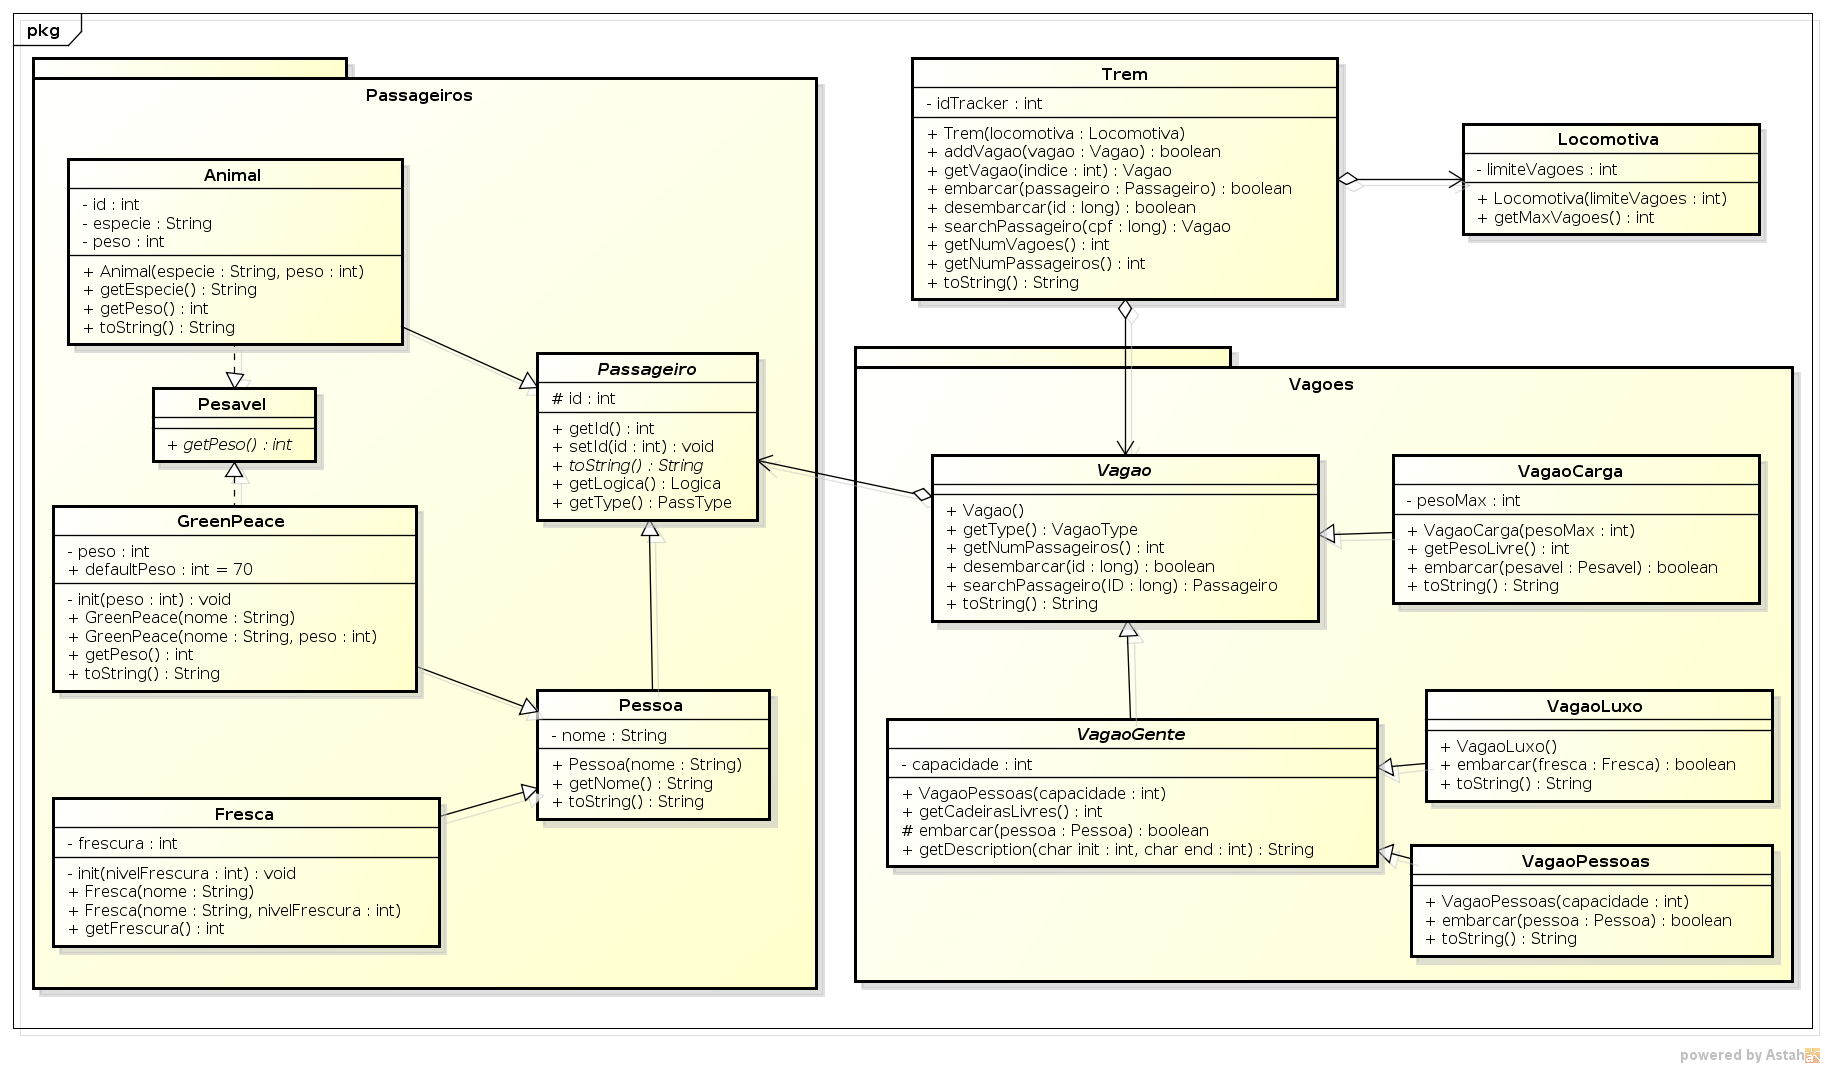
\includegraphics[width=1\linewidth]{./diagrama}
\caption{Diagrama de Classes}
\label{fig:diagrama}
\end{figure}
%\end{sidewaysfigure}
\end{landscape}


\begin{lstlisting}[float =ht, label=output, caption=Saida Esperada]
Trem{
    [ 0:Cao:20  _:15 ]
    ( 2:Gr2:40 4:Do )
    [ 1:Gr1:70  _:0 ]
    ( _ _ )
    ( _ _ )
    ( 7:F3 _ )
    [  _:10 ]
    @ 5:F1 6:F2 @
}

\end{lstlisting}

\lstinputlisting[label=controlador, caption=Controlador, float=ht]{controlador.java}

\end{document}
